\documentclass[12pt]{article}

\setlength{\topmargin}{-.75in} \addtolength{\textheight}{2.00in}
\setlength{\oddsidemargin}{.00in} \addtolength{\textwidth}{.75in}

\usepackage{amsmath,color,graphicx,array,multirow,rotating, enumerate}
\usepackage{type1cm}
\usepackage{eso-pic}
\usepackage[hmargin=2cm,vmargin=1.3cm]{geometry}
\usepackage{mathabx}
\usepackage[rflt]{/Users/jgates/desktop/latex/floatflt}
\usepackage[table]{xcolor}
\nofiles

\def\Tab#1{\tabular[t]{>{\rule[-1ex]{0pt}{3ex}}c}#1\endtabular}
\newcolumntype{C}{@{}c@{}}

\pagestyle{empty}
\newcounter{ProbNum}
\setlength{\parindent}{0in}

% Watermark: graph paper
\newcommand\BackgroundPic{
\put(0,0){
\parbox[b][\paperheight]{\paperwidth}{%
\vfill
\centering
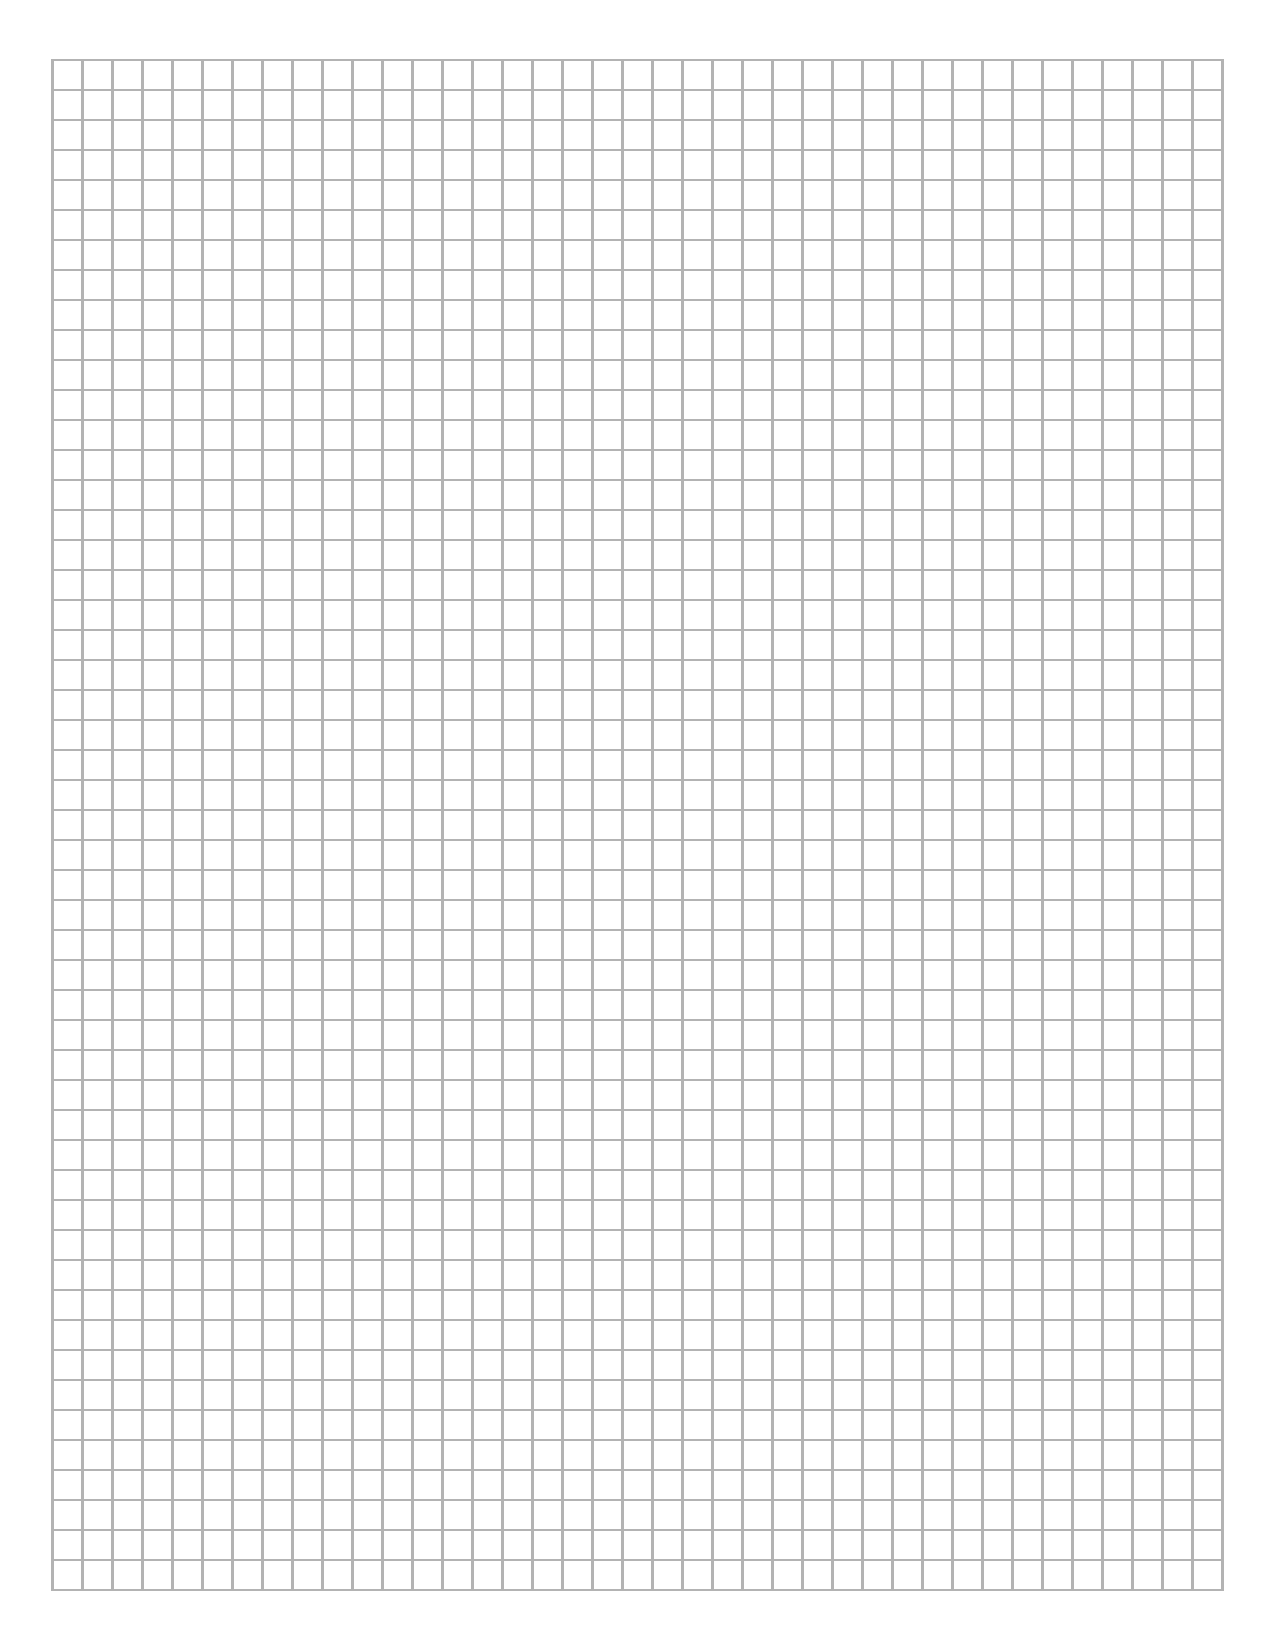
\includegraphics[width=\paperwidth,height=\paperheight,keepaspectratio]{/Users/jgates/desktop/latex/pics/plain.pdf}%
\vfill
}}}

%Diagram box command [v space][content]
\newcommand{\diagrambox}[2][40 mm]{
\framebox{\parbox{175 mm}{#2 \hfill \\ \vspace{#1}}}

\bigskip
}

% MakeList: [example number] [content]
\newcommand{\MakeList}[2]{
\begin{enumerate}[#1] \itemsep1pt \parskip0pt \parsep0pt  

#2
\end{enumerate}
}

\begin{document}



{\Large Problems tagged with standards:}KFriction
\bigskip 
% Number 20
% UFPM CAPM Friction KFriction 
% Box sliding down frictionless incline: a, motion

% Watermark
\AddToShipoutPicture*{\BackgroundPic}

\addtocounter {ProbNum} {1}

\begin{floatingfigure}[r]{.25\textwidth}
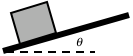
\includegraphics{/Users/jgates/desktop/latex/pics/incline1.png}
\end{floatingfigure} 

{\bf \Large{20.}} A box of mass ${m}$ slides with an initial velocity of ${3~\tfrac{m}{s}}$ down a ramp which is inclined ${20^\circ}$ from the horizontal.  The coefficient of kinetic friction between the ramp and box is .45.

\bigskip

\indent  a. Determine the direction and magnitude of the acceleration of the box as it slides down the incline. 

\bigskip 
b. Discuss the subsequent motion of the box (qualitatively - no numbers are necessary).

\bigskip 
\vspace{6mm}% Number 530
% UFPM SFriction KFriction Algebra Units CAPMA
% Sliding crate on truck bed - friction
% KO

% Watermark
\AddToShipoutPicture*{\BackgroundPic}

\addtocounter {ProbNum} {1}

%\begin{floatingfigure}[r]{.45\textwidth}
%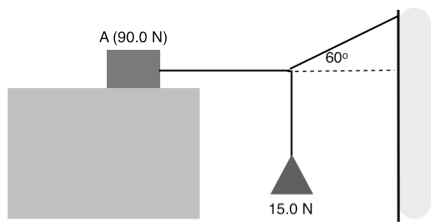
\includegraphics[scale=.6]{/Users/jgates/desktop/latex/pics/static1}
%\end{floatingfigure}
 
{\bf \Large{530.}} A 20 kg box rests on the flat floor of a truck. The coefficients of friction between the box and floor are ${\mu_s=.15}$ and ${\mu_k=.1}$. The truck stops gently at a stop sign and then starts to move with a constant acceleration. The box is 2.2 m from the rear of the truck when the truck starts.

\bigskip
What is the maximum possible acceleration that the truck may have if the box is not to slide?

\bigskip Suppose that the acceleration of the truck is instead ${2.1~\tfrac{m}{s^2}}$. How much time elapses before the box falls off the rear of the truck? 

\bigskip How far does the truck travel in this time?

%\hfill 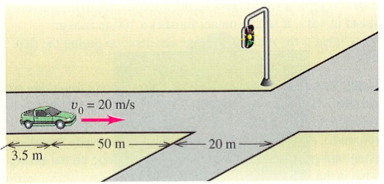
\includegraphics[scale=.85]{/Users/jgates/desktop/latex/pics/redlight.png}


\bigskip \vspace{6mm}% Number 550
% UFPM SFriction Algebra Units CAPMA KFriction
% Block held up to vertical cart by acceleration/friction
% KO/JG

% Watermark
\AddToShipoutPicture*{\BackgroundPic}

\addtocounter {ProbNum} {1}

\begin{floatingfigure}[r]{.2\textwidth}
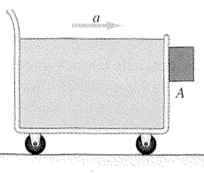
\includegraphics[scale=.6]{/Users/jgates/desktop/latex/pics/cartstatic}
\end{floatingfigure}
 
{\bf \Large{550.}} The cart accelerates to the right, keeping block A from sliding down. The coefficient of static friction between the block and the cart is .8, and the coefficient of kinetic friction is .5. The block is 1.2 meters above the ground.

\bigskip
What minimum acceleration must the cart have in order that block A does not fall? 

\bigskip If the acceleration of the cart were only half that value, how long would it take for the block to hit the ground?
%\hfill 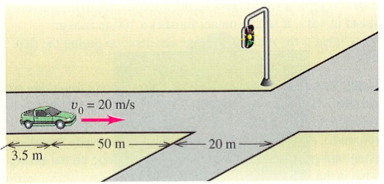
\includegraphics[scale=.85]{/Users/jgates/desktop/latex/pics/redlight.png}

\bigskip \bigskip \vspace{6mm}% Number 640
% BFPM Tension KFriction
% Half Atwood - sliding at const. v
% JG

% Watermark
\AddToShipoutPicture*{\BackgroundPic}

\addtocounter {ProbNum} {1}

\begin{floatingfigure}[r]{.2\textwidth}
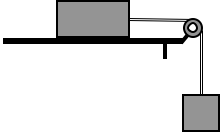
\includegraphics[scale=.6]{/Users/jgates/desktop/latex/pics/halfatwood3}
\end{floatingfigure}
 
{\bf \Large{640.}} A 2 kg box sits on a rough (non-frictionless) table. It is connected by a massless string to a hanging 1 kg box.  If I give the box a short push to start it moving to the left, it will slide at a constant speed.
 
\bigskip
What is the coefficient of kinetic friction between the box and the table?\paragraph{}
\noindent
\bigskip 
%\hfill 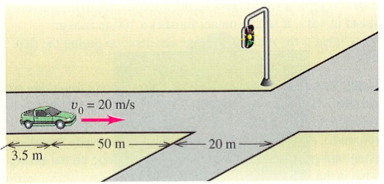
\includegraphics[scale=.85]{/Users/jgates/desktop/latex/pics/redlight.png}
\vspace{6mm}% Number 710
% CoPM CoEM KFriction Algebra Units Vectors
% Bullet/block: inclined plane- friction and frictionless
% MIT/JG

% Watermark
\AddToShipoutPicture*{\BackgroundPic}

\addtocounter {ProbNum} {1}

\begin{floatingfigure}[r]{.42\textwidth}
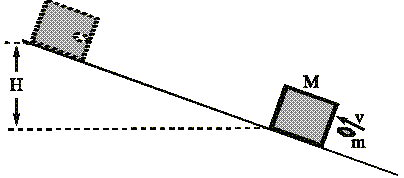
\includegraphics[scale=.6]{/Users/jgates/desktop/latex/pics/inclinebulletblock}
\end{floatingfigure}
 
{\bf \Large{710.}} A bullet of mass $25~g$ is fired along an incline and imbeds itself quickly into a block of wood of mass $2.5~kg$. The block and bullet then slide up the frictionless $20^{\circ}$ incline, traveling a maximum distance of 3.5 meters up the incline. The block is kept from sliding down the incline initially by as small peg (not shown).

\bigskip
Determine the speed of the bullet just before it hits the wood.\paragraph{}
\noindent
\bigskip 
Suppose instead that the incline is not frictionless, and that there is a coefficient of kinetic friction between the incline and the block of .2.  Determine how far the block travels up the ramp in this situation. 
\bigskip %\hfill 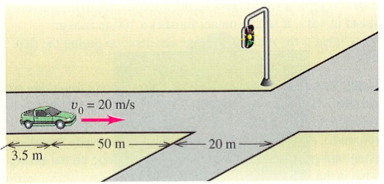
\includegraphics[scale=.85]{/Users/jgates/desktop/latex/pics/redlight.png}
\vspace{6mm}\end{document}